\chapter{Epidemics and Influence Maximization in Complex Networks}
\label{cha:2}
Influence Maximization is an algorithmic problem in complex networks \cite{SINGH20227570}. The problem consists of finding the best Seed Set K of a Network so that the spread of influence is maximized at the end. We are interested in maximizing the number of total influenced nodes.
This makes social influence problems very important since their range of application is enormous, going from viral marketing to disease and fake news epidemic spread. A good example of practical application in Viral Marketing is choosing the best influential users on the social network to endorse a product, to maximize the interest in that product across the whole network. What follows is an analysis of the related works on influence maximization that inspired this thesis. \\
Studies on clusters like \cite{articl2e} are extremely useful for the characterization of the network and feature extraction, useful for developing solutions for specific algorithmic problems. The work that mostly inspired this thesis is the study by Sirag Erkol et. al \cite{unknown} that extends the common greedy algorithm for static network influence maximization to a temporal perspective. This work is based on a similar infection model, but oriented towards a more realistic and less optimal direction that can better fit a realistic situation.
\\
 
\section{SI Model}
\label{sec:si}
The network is modeled through a Susceptible-Infected model
\cite{MORE2019102}. That is the simplest form when talking about disease models, since it does not include recover dynamics, but for the sake of IM those are just random probabilities that limit the overall performance, but do not play any key role when selecting the best initial Seed Set. It also allows spreading on single interactions, unlike models where the influence only affects a node based on how much the same influence is spread among his neighbors.
In a SI model every node is either in a Susceptible (neutral) or Infected state, and cannot revert once it enters the second one. Every node is Susceptible at time zero, except the Seed Set nodes that are set to Infected. Every time an Infected node interacts with a Susceptible one according to the network there is a fixed probability Pspread of that second node becoming Infected as well. On the current implementation an eventual failure of spreading between two nodes does not affect the second node's probability of being infected in the future (fixed probability).
Future works aim at extending the simulation context by adding recover dynamics and also dynamic probability and trust dynamics between nodes.

\begin{center}
    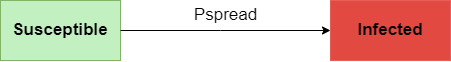
\includegraphics[scale=1]{simodel}
\end{center}


\begin{center}
    Figure 2.1: Susceptible-Infected Model
\end{center}

\section{Related Work and Optimal Solutions}
\label{sec:litreview}
Influence maximization has been widely studied since it's extremely important to identify the most influential seed set in a complex network. Optimization solutions have been proven to be NP Hard, the goal of this work is to measure and compare the performance of quicker and possibly sub-optimal solutions under more realistic circumstances not considered in existing works. 

\subsection{SI Influence Maximization On Static Networks}
\label{sec:static}

Most of the existing work on influence maximization is based on the assumption of the network being static. The optimization algorithm is greedy \cite{article}, and gradually builds the Seed Set by adding the node that can better improve the influence spread of the current Seed Set; this can be either calculated or estimated each time, meaning that the algorithm will be NP-Hard. Quicker algorithms that can give good performance can be built on the same greedy base but using easier graph concepts to estimate a node’s influence, for example degree centrality. 
The work proposed deals instead with dynamic (or temporal) networks, that can represent a social network in a better way considering the fact that not every user is connected at the same time.

\subsection{SI Influence Maximization On Temporal Networks}
\label{sec:dynamic}
Many studies of Influence maximization are limited to static networks that do not change through the time; this can be restrictive because often interactions change over time in a highly dynamic manner. The optimization solution in temporal networks is a natural extension of the greedy algorithm for static networks\cite{unknown}, however when working with non-optimal solutions, like this work does, it is not possible to predict exactly how much a node is going to contribute to influence. That is because influence starts from a Seed Set but is then propagated through a cascade based on the interaction between the nodes. Furthermore, in temporal networks the cascade follows some time order, meaning that there are nodes that activate earlier than others, so in those scenarios it is not only important to consider the “popularity” of a node, but also how it can impact the whole cascade. Notice that, in order to analyze that aspect, full knowledge about the network (nodes, size) and its evolution is needed, otherwise it is essential to implement algorithms to predict the network changes. In a study by H. Zhuang et. al \cite{inproceedings} are proposed some algorithms to probe the network at a time t with no knowledge and predict the full network structure at that time by reconstructing it through the probing data and the information about the previous stages. However, this dissertation is based on having full network knowledge, and will take into account all the just discussed variables, that depend on the network structure, combining them with realistic general influence variables such as a limited budget, cost of selecting an initial node, and spreading probability.

\subsection{Seed Set and Cost}
\label{sec:dycost}
Most of the existing works on influence maximization aim at finding a generally small number of initial nodes, by setting a maximum cardinality k to the initial Seed Set and building it gradually through greedy approaches. This makes seed sets to be all made of k nodes, with chosen nodes being characterized by the different solution algorithms.  When trying to expand seeding to a more realistic scenario, it is inevitable to give each node a different cost depending on his role inside the network. Viral Marketing is a clear example of that, where we obviously need more budget to make some product be advertised by some famous influencer(s).
This works proposes dynamic costs for each node, depending on his degree in the network, and a fixed budget cap is introduced. This allows the seeding to be more realistic and various in both size and nodes selected. The idea here is that the more a network node is influent (interacts with other nodes) the more his cost to be initially selected grows. This is why the exponential function is used to dynamically compute the cost of a node, this way nodes with higher degree are always going to be out of budget, encouraging the usage of more marginal nodes to see how well they can do based on the network structure.
The cost of a node n is calculated as follows:
\begin{center}
    $c(n) = {\rm e}^{\delta(n)} \, ,$
where $c(n)$ is the cost of node $n$, and $\delta(n)$ is its degree
\end{center}
Note that this also never allows a node's cost to be zero.
\\
Depending on the structure of the network (number of nodes, edges) different simulations with growing budgets are performed for each strategy to measure how good it works. The goal of this work is to study how far we can spread our influence on different networks with extremely limited budget.

\subsection{Network Knowledge}
\label{sec:input}
This dissertation, along with almost all the existing works on influence maximization, works on the assumption that full network knowledge is given, as well as full information on when and how it evolves through the time. 

\section{Proposed Work}
\label{sec:proposed}
The dissertation will bring an unique realistic aspect when developing a seeding strategy on a complex temporal network. It will cover the temporal aspect of the network, as well as a constraint on the maximum budget available to select the nodes to be infected at the beginning. The  network is modeled with a Directed Graph, and a classic SI model is used for influence maximization, hence the influence happens through the interaction between different nodes in the network, starting from the selected K initial nodes. Furthermore, this work aims at proposing and measuring the performance of non-optimal strategies that can be applied to large-scale realistic networks under severe budget restrictions.







